\documentclass{article}

\usepackage{fontspec}

\usepackage{todonotes}

\usepackage[xetex, colorlinks=true]{hyperref}
\usepackage[
   backend=biber,
   bibencoding=utf8,
   style=alphabetic,
   hyperref=true,
   % citestyle=authoryear-comp,
   backref=false,
   sortlocale=en,
   url=true,
   doi=false,
   eprint=false
 ]{biblatex}
\addbibresource{biblio.bib}

\newcommand\Coq{Coq}
\newcommand\OCaml{OCaml}
\newcommand\R{R}
\newcommand\Cn{C}

\usepackage{minted}
\setminted{encoding=utf8}

\usepackage{tikz}
\usetikzlibrary{positioning}

\tikzset{
	box/.style = {
		draw = black,
        fill = white,
		rectangle,
		rounded corners = 2pt,
		text centered,
		minimum height = 5mm,
		minimum width = 10mm
	}
}

\newcommand\mod{\mathit{mod}}


\title{Notes about \R}
\author{Martin Bodin}

\begin{document}

\maketitle

\section{Presentation of the Language}
\label{sec:presentation}

\R{} is now a trending programming language for mathematicians.
In practise, it is presented as a read-eval-print-loop,
but it is also possible to write programs in it.
% The language enables easy integration of \Cn{} functions.
The language presents itself as a weakly typed programming language
manipulating different types of arrays.
The syntax of the language contains numerous exceptions,
leading to a high number of programs with a semantics.

\subsection{History}
\label{sec:history}

\R{} is a programming language designed for statistics.
Its specification~\parencite{team2000r}\footnote{
    This specification is also given directly in \R{} itself,
    by typing \mintinline{R}{help.search ()},
    and clicking of the “\R{} Language Definition” link
    on the webpage then opened.
} is not precise (but really helps understand \R{} source code):
in practise, it is specified by its main implementation~\parencite{Rwebsite}.

The original authors of \R{}~\parencite{ihaka1996r}
describe \R{} as a programming language similar to Scheme
which has been mutated to get a programming language similar
in appearance and features to S.
In particular, \R{} features scoping and first-class functions
as Scheme
(whereas in S, nested functions are not lexically scoped).
Similarly to S, however, it is a lazy programming language.

It is a community driven programming language.
This means that most of what is used in a \R{} program comes from various libraries,
which can change the way the programming language behaves.
This can be compared with JavaScript,
and how libraries like jQuery changes the way programs look.
However, not all of these libraries are written in \R{}:
some are written in \Cn{} or Fortran
with an interface in \R{}.

One of the reasons of the success of \R{}
is its built-in help system.
Each functions are documented with examples
and can be accessed by typing in \R{}
a question mark followed by the corresponding feature.
For instance \mintinline{R}{?c} displays
the documentation of the \mintinline{R}{c} function,
and \mintinline{R}{?'<-'} displays the documentation
of the \mintinline{R}{<-} feature.

\subsection{Features}
\label{sec:features}

\R{} is accompanied with a lot of features.
We detail here the ones relevant from the point of view
of it as a programming language.

\subsubsection{Promises}
\label{sec:promises}

The \R{} programming language is lazy.
This was a design choice:
it is frequent in \R{} to define a large array,
but then filter it to only consider a small number of its cells.
Lazyness enables the programming language to focus on these cells
and only compute what is needed to display their content.

In practise, lazyness comes in the form of promises.
A promise is composed of a syntactic expression,
an environment, and an optional value.
If \R{} needs the result of promise,
it will check the optional value.
If it is present, the promise already has been computed
and the value is directly reused.
Otherwise, the promise's expression is evaluated,
and the promise's value is set to the returned value.
The evaluation of the expression might raises side effects.
%
A typical place where promises are defined
is during function calls.
\begin{minted}{R}
f <- function (x, y)
     if (x == 1) y
# “f” is now a function
f (1, 2 + 2) # The expression “2 + 2” becomes here a promise.
# The function “f” uses this promise, and it thus reduces to “4”.
f (1, a <- 1) # This promise has a side effect.
a # Returns 1. Note that the promise kept the initial environment:
  # the variable “a” has been defined in the initial environment.
f (0, b <- 1) # This promise has a side effect, but is not evaluated.
b # Returns an error.
\end{minted}

This lazyness feature of \R{} enables
language constructs like \mintinline{R}{if}
to be considered as \emph{functions}.
There are thus very few cases in the evaluation function
of \R{}, corresponding to the atomic types.
This also enables libraries to drastically change
the language's syntax.

Function arguments can have default argument,
but in this case, it is still a promise.
In the following example,
the variable \mintinline{R}{y} is associated with
the promise \mintinline{R}{x} and the local environment
of the call (not the one from the calling point).
But this environment may change during the function evaluation.
\begin{minted}{R}
x <- 1 # A global variable.
f <- function (x, y = x) { # The variable “y” receives the promise “x”.
       x <- 3 # We update the variable “x”.
       y      # Evaluates the promise.
       x <- 4 # We update again “x”.
       y      # The promise has already been evaluated.
     }
f (2) # The local variable “x” is set to 2.
# Returns 3.
\end{minted}

One of the initial goals of the \R{} programming language
was to provide easy visualisation tools,
through functions like \mintinline{R}{plot},
drawing a graph.
To express equations, we can in \R{} uses promises.
Here is an example taken from the original paper~\parencite{ihaka1996r}.
\begin{minted}{R}
curve <- function (expr, from, to) {
           x <- seq (from, to, length = 500)
           y <- eval (substitute (expr))
           plot (x, y)
         }
\end{minted}
This function can be invoked as
\mintinline{R}{curve (x^2 - 1, -2, 2)}
to draw the function \(f(x) = x^2 - 1\)
over the interval \([-2, 2]\).
We now describe what happens during
this call.
First, the variable \mintinline{R}{expr}
is associated with he promise \mintinline{R}{x^2 - 1}
in the initial environment.
This may be seen strange as the initial environment
does not define any variable \mintinline{R}{x}.
Inside the scope of function \mintinline{R}{curve},
a variable \mintinline{R}{x} is defined, as a vector.
The function \mintinline{R}{substitute} is a special function,
as it manipulates the inner data type of the promise \mintinline{R}{expr}:
it replaces its inner environment with the current environment
(that is, the inner scope).
The variable \mintinline{R}{x} inside the promise
\mintinline{R}{expr} is now linked with the local
variable \mintinline{R}{x},
and the promise can be evaluated.


\subsubsection{Vectors}
\label{sec:vectors}

In the previous example,
the variable \mintinline{R}{x} was associated the result
of \mintinline{R}{seq}, which is a numerical vector.
It can be surprising be able to compute
the expression \mintinline{R}{x^2 - 1},
as \mintinline{R}{x} is not a number.
The reason is that the operators \mintinline{R}{^} and \mintinline{R}{-}
applies on vectors, component by component.
The numbers \mintinline{R}{2} and \mintinline{R}{1}
in the expression are seen as vectors with only one cell.
We cannot assign a variable to a number,
but we can assign it a numerical vector of size one,
and \R{} does it all the time.
As the vectors \mintinline{R}{2} and \mintinline{R}{1}
are not the same size than \mintinline{R}{x},
their values are reused in a cyclic manner.
In most cases, this is what the user wants,
but it can be surprising if the user thought that both
vectors had the same size but had not:
no warning will be emitted by \R{}.

One operation whose semantics can be difficult
to fully comprehend is the vector indexing.
Given a vector \mintinline{R}{v},
we can filter it by \mintinline{R}{v[i]}.
The behaviour of this operation will be very different,
depending on the nature of \mintinline{R}{i}.
\begin{itemize}
    \item If \mintinline{R}{i} is a logical vector\footnote{
          Logical vectors stores tri-valued booleans,
          which can be \mintinline{R}{TRUE}, \mintinline{R}{FALSE},
          or \mintinline{R}{NA} (not applicable).
          All base values have an \mintinline{R}{NA} value.
      }, then \mintinline{R}{i} is first repeated
      to match the size of \mintinline{R}{v}.
      Then, each index of \mintinline{R}{v} corresponding
      to the value \mintinline{R}{TRUE} from the index array \mintinline{R}{i}
      are conserved;
      each corresponding to \mintinline{R}{FALSE} are removed;
      and each corresponding to \mintinline{R}{NA} are replaced
      by the \mintinline{R}{NA} of the expected type.
    \item If \mintinline{R}{i} is a numerical vector,
      and that all its elements are positive, zero, or \mintinline{R}{NA},
      then the corresponding indices of \mintinline{R}
      are taken in the given order, resulting in an array
      that can be thought of the same size than \mintinline{R}{i}.
      Indexes of \mintinline{R}{v} are however counted from
      \(1\), and all \(0\) in \mintinline{R}{i} are ignored.
      If \mintinline{R}{i} contains \mintinline{R}{NA},
      they yield \mintinline{R}{NA} in the resulting array.
      Values of \mintinline{R}{i} greater than the size of \mintinline{R}{v}
      results in \mintinline{R}{NA}.
        Note that a special case of this case is when the size of \mintinline{R}{i}
      is one (as in \mintinline{R}{v[18]}),
      \R{} then returns an array with only one cell,
      which looks like a base value.
    \item If \mintinline{R}{i} is a non-empty numerical vector
      whose elements are all negative or zero,
      then the result is the array \mintinline{R}{v}
      in which all values whose index (starting from \(1\))
      is the opposite of a number in \mintinline{R}{i} are removed.
    \item If \mintinline{R}{i} is a vector of character strings,
      and that \mintinline{R}{v} is associated with a \mintinline{R}{names}
      attribute\footnote{
          Any \R{} object can be associated attributes.
          They are a simple name to value mapping,
          which can be updated at will.
      }.
      We do not detail this case in details,
      but \R{} then intuitively selects the cells of \mintinline{R}{v}
      by their names.
\end{itemize}

As an example, if \mintinline{R}{x} is a vector of numbers,
then \mintinline{R}{x < 0} is a vector of booleans
(\mintinline{R}{<} is an operation applying on the components
of a vector, and the vector \mintinline{R}{0} is repeated).
As a consequence, \mintinline{R}{x[x < 0]} is the subvector of
\mintinline{R}{x} containing only its negative values.
This is often used in the left-side of an assignment\footnote{
    The left side of expression can be a variety of things,
    not just variables.
    It is however a complex operation with a lot of corner cases,
    and I prefer not to explain it in detail in this document.
}, as in \mintinline{R}{x[x < 0] <- 0} which replaces all
negative values of \mintinline{R}{x} by \mintinline{R}{0}.

\subsubsection{Function Calls}
\label{sec:function:calls}

The part of \R{} source code dealing with function application,
and in particular in the part matching the given argument to the
expected (formal) arguments, is surprisingly long.
The reason is that there are several, separately simple, ways to call
a function.
Each of these ways then interoperate in each call,
making them sometimes quite complex.

We have seen in Section~\ref{sec:promises} that default arguments can be given
to a function argument:
if the argument is not provided, a promise is associated with the default expression.
Arguments can also be given by name,
as in the \mintinline{R}{curve} example of the same section:
the function \mintinline{R}{seq} is given its argument named \mintinline{R}{length}
as a named argument,
overwriting the argument order.

Arguments can also be missing.
This does not break the function call.
However, if the associated promise is evaluated, then an error is thrown.
However, we can not provide more arguments than what a function expects,
resulting in an error during the function call.
It is however possible to provide a \mintinline{R}{...} formal argument
to a function definition.
When called, all additional arguments will be packed in a special array.

Surprisingly, named arguments are matched by prefix
(called “partial match” in \R{} source code) and not only by exact name,
unless they are after a \mintinline{R}{...} formal argument.
For instance, in the example below,
we can refer to the argument \mintinline{R}{cd} as just \mintinline{R}{c}.
Exact matches have however higher priority to prefix:
although \mintinline{R}{ab} is a prefix of \mintinline{R}{abc},
as it exactly corresponds to the name of a formal argument,
\R{} do not mix them.
Also, exact matches are checked first, and partial matches second:
this is the reason why the call \mintinline{R}{f (ab = 2, a = 1, 3)}
below succeeds, assigning \mintinline{R}{abc}
(and not \mintinline{R}{ab}) to \(1\).
\begin{minted}{R}
f <- function (abc, ab, de) c (abc, ab, de)
# All the expressions below returns the array 1 2 3.
f (1, 2, 3)
f (de = 3, 1, 2)
f (d = 3, 1, 2)
f (ab = 2, 1, 2)
f (ab = 2, a = 1, 3)
f (a = 3, 1, 2) # Returns an error, as “a” is the prefix of several formal arguments.
\end{minted}


\section{\R{} Interpreters}
\label{sec:interpreters}

There are several interpreters of \R{}.
One is the official implementation,
but others exist (mainly to provide more speed).

\subsection{The Main \R{} Interpreter}
\label{sec:main:interpreter}

\subsubsection{Concepts}
\label{sec:concepts}

Most \R{} objects are in the form of a \emph{basic language element}.
This is a \Cn{} structure composed of a tag and four pointers.
The tag indicates the kind of the basic language element;
it can be for instance an integer vector, an environment, an expression, or an external pointer.
The first pointer is used to associate \emph{attributes} to the basic language element.
Attributes are additional fields that can be added to almost any \R{} object;
they are untyped.

The meaning of the last three vectors depends on the flag.
%
For instance, for an environment, the first (data) pointer is a pointer
to the current frame (associating each local variable to a value or a promise),
the second pointer points to the environment of the outer scope,
and the third pointer points to a hash (to enable faster checks).
%
For a list, the first pointer points to the first element of the list,
the second, to the rest of the list,
and the third, to an optional name for the first element.

Vectors are specials.
They are associated with the same tag and attribute pointer
than other basic language elements,
then two integers follow.
Lastly, a raw array of data directly follows the basic language element in the \Cn{} memory.
The two integers store the size of this array as well as its allocated size
(which is usually the same than its current size).
The size of this array’s cells depend on what it stores
(indicated by its tag):
for a character vector, it will be an array of characters,
for an integer vector, an array of integers, etc.


\subsubsection{Main Files and Functions}
\label{sec:files}

This table shows the various main files of the \Cn{} source code of \R{}.

\begin{tabular}{|c|p{7cm}|}
    \hline
    \texttt{src/include/Internal.h} & Defines the basic language element structure. \\
    \hline
    \texttt{src/main/names.c} & Fills in the global environment, associating each \R{} construct/name to its corresponding \Cn{} function. \\
    \hline
    \texttt{src/main/eval.c} & Defines \Cn{} functions to evaluate expressions. In particular the function \mintinline{C}{eval}, taking an expression and an environment and evaluating the expression. \\
    \hline
    \texttt{src/main/match.c} & Contains various function to deal with the association between formal and given arguments in a function call. \\
    \hline
    \texttt{src/main/context.c} & Defines contexts, which is a structure used to manipulate informations relative to program points, for constructs like \mintinline{R}{break} or \mintinline{R}{return}. \\
    \hline
    \texttt{src/main/envir.c} & Defines various \Cn{} functions to manipulate environments. \\
    \hline
    \texttt{src/main/coerce.c} & Contains a \Cn{} functions to converts \R{} values to other types. It also contains the \mintinline{R}{substitute} function. \\
    \hline
\end{tabular}

These files change regularly,
but rarely in the \Cn{} part.
Most of the changes between the current (trunk) version
and in Version~\(3.0\) (from 2012, that is five years ago)
are changes in the preprocessor
(some architectures includes different headers),
added documentation in comments,
small type changes between similar types
(\mintinline{C}{unsigned long} updated to \mintinline{C}{size_t}),
code restructuration,
and more importantly,
new behaviours.
There new behaviours are mostly additional checks
and exceptions providing more behaviours
(or more precise behaviours) to the \R{} interpreter
for rare cases.

\subsubsection{Optimisations}
\label{sec:optimisations}

The main \R{} interpreter is written with various optimisations in mind.
This section lists some of them.

\paragraph{Symbols as Pointers}
%
Comparing strings is costly,
and variables are inherently stored as strings.
The main \R{} implementation,
fixes this costly operation by comparing pointers
instead of strings.
First, any symbol must be installed using the \mintinline{C}{install}
function, defined in \texttt{src/main/names.c}.
This function allocates a basic language element
of type “symbol”.
One of its pointer points to the associated string.
Then the pointer to this basic language element
is always used instead of the initial string.
%
Symbols are stored in a global hash table:
when “installing” a new symbol, it is first checked
that the symbol did not already exist:
if so, we have to return the previously allocated pointer.


\subsection{FastR}
\label{sec:FastR}

The \R{} runtime can be slow.
\cite{kalibera2014fast} propose a faster approach,
based on a Java implementation.
This implementation is itself based on the Truffle
framework~\parencite{wimmer2012truffle}.
This framework aims to build an optimised virtual machine
from an unoptimised interpreter in Java.
It is based on code specialisation,
compiling each functions into several versions,
depending on the types of its arguments.

Due to the framework (as well as the Java virtual machine),
FastR needs some time to “warm-up” and get to its full speed.
During this initialisation, it can be slower than the main
\R{} interpreter.
However, once it gets to a critical loop,
it is usually much faster than the main \R{} interpreter.

\subsection{TestR}
\label{sec:TestR}

TestR is a framework to generate and execute unit tests.
It also aims at measuring the coverage of the generated tests
in the main interpreter source code,
as well as in its various \R{} libraries.

Although not an interpreter,
this test suite can be considered as a trust source
for my \Coq{} formalisation of the \R{} programming language.


\section{Formalisation}
\label{sec:formalisation}

This section describes my approach to formalise \R{} in \Coq{}.

\subsection{Language Formalisation}
\label{sec:language:formalisation}

Following my experience with JSCert~\parencite{bodin2014trusted},
I think that it is important to have a specification
the closest possible to \R{} internals.
Indeed, JavaScript manipulates structures somehow similar
to the basic language elements of \R{} (see Section~\ref{sec:concepts}),
called completion triples.
In JSCert, we initially choose to represent these completion triples
as a \Coq{} inductive,
each case of the triples only containing the attributes that made sense for us.
For instance, a basic language element whose tag is “symbol”
will probably only use one pointer to represent the string of the symbol.
By we discovered later that a construct of JavaScript % The sequence
broke what we thought were invariants:
the standard manipulated the structure as if it was a \Cn{} structure
(and not as a usual pseudo-code structure),
breaking our type assumptions.
We were forced to start the formalisation again with a structure
closer to the standard.

I thus propose a formalisation based on the structure below.
Arrows represent trust relations,
those which are dashed are planned but not yet implemented.
It is inspired by the refinement methodology~\parencite{cohen2013refinements}:
produce several implementations,
one easier to specify and one easier (or more efficient) to implement,
then prove correct each one relatively to the next one.
\begin{center}
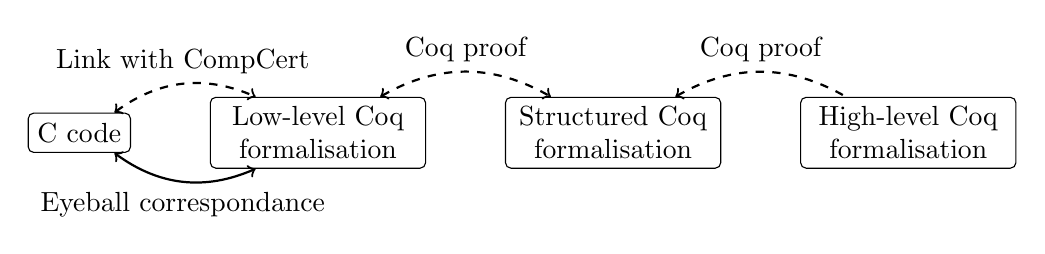
\begin{tikzpicture}
    \node [box] (C) {\Cn{} code} ;
    \node [box, right = 1cm of C] (low) {\parbox{25mm}{\centering{}Low-level \Coq{} formalisation}} ;
    \node [box, right = 1cm of low] (structured) {\parbox{25mm}{\centering{}Structured \Coq{} formalisation}} ;
    \node [box, right = 1cm of structured] (intuition) {\parbox{25mm}{\centering{}High-level \Coq{} formalisation}} ;

    \draw [<->, thick, dashed] (C) to [bend left] node [above] {Link with CompCert} (low) ;
    \draw [<->, thick] (low) to [bend left] node [below] {Eyeball correspondance} (C) ;
    \draw [<->, thick, dashed] (low) to [bend left] node [above] {\Coq{} proof} (structured) ;
    \draw [<-, thick, dashed] (structured) to [bend left] node [above] {\Coq{} proof} (intuition) ;
\end{tikzpicture}
\end{center}
At one end of the refinements is the \Cn{} source code of the \R{} interpreter.
As \R{} is defined by implementation,
this can be seen as a specification.
We in particular focus on the parts defining program evaluation
(mostly the files \texttt{src/include/Internal.h} and \texttt{src/main/eval.c}),
ignoring most constructs of the \R{} programming language.
A \Coq{} version of these \Cn{} definitions is defined,
with the aim to be the closest possible to the \Cn{} definition.
Some parts of the functions are dropped at this level,
such as error management.
At term, it is planned to use CompCert~\parencite{Leroy-Compcert-CACM}
(or any other \Coq{} semantics of \Cn{}~\parencite{formalin})
to prove that the \Coq{}
version is indeed identical to the chosen parts of the \Cn{} definition.

A structured \Coq{} formalisation is then defined.
This formalisation abstracts some low-level constructs,
such as pointers to basic language elements
(which are heavily used in \R{}'s source code).
In particular, this version should abstract all what can be abstracted
about the memory model:
most pointers to basic language elements
will be replaced by a \Coq{} inductive representing
the corresponding basic language element.
As \R{} semantics is mostly functional
(with the exception of environments),
this step should not raise too much difficulty.
The basic language elements are also given a proper
inductive at this stage (representing \R{} expressions),
although it is only weakly typed.
Abstracting the memory enables to make explicit
a subtlety of \Cn{} pointers,
which can be used for two distinct usages:
a pointer to one object,
or a pointer to an array of this object.
In this structured formalisation, the pointers to arrays
are replaced by a list,
which is much easier to manipulate in \Coq{}.

The last step of the process aims to fit
the intuition that the original authors had in mind when defining
the \R{} programming language~\parencite{ihaka1996r},
which hopefully fits the intuition of programmers.
As such, this third formalisation can also be considered to be a trust source.

These formalisations are chosen to be interpretable.
This enables to add another trust source
by running these interpreters against \R{} test suites.
Code coverage can also be applied on the extracted \OCaml{} interpreters
using tools such as Bisect.

One of the reasons why \R{} is so accurate for such a formalisation choice
is its modularity:
these three formalisations focus on the core of \R{}.
Most of the additional features of \R{} can then be iteratively be added.
For instance, the assignment feature \mintinline{R}{<-} is not
strictly speaking in the core of \R{} and can be later added.
These additional features can be limited to the ones needed to analyse
a given program:
it is not needed to formalise the entire \R{} programming language to start
using these formalisations.
In this aspect, \R{} is modular.
%
This also means that some features of \R{} can be formalised
in less details than others
without altering the trust of the code formalisation.

We now discuss the proofs of equivalence between \Coq{} formalisations.
%
The first proof is between the low-level formalisation
and the structured level one.
The main change between the two formalisation is the memory model.
As such, there are no semantic changes,
and they can (at least in theory)
be proven equivalent.
However, the deterministic aspect of the formalisation
(as both are \Coq{} interpreters)
simplifies the equivalence proof:
only one direction\footnote{
    That is, that if one formalisation results in something,
    then so does the other.
} is needed to get the equivalence.
%
The second proof, between the structured formalisation
and the high-level is more complex.
Indeed, the high-level formalisation manipulates
different structures than the structured one.
Furthermore, the high-level structures carry assumptions:
some advanced \R{} constructs may not fit such a high-level formalisation,
for instance because they manipulate low-level bits or fields.
If the assumptions underlying the high-level formalisation
are broken, no result is given in the high-level semantics;
but this doesn’t mean that there is no accepted results in the
structured formalisation, which assumes less.
The proof of correctness between these two formalisation
is thus bound to be in only one direction:
if the high-level returns a given result,
so does the structured formalisation.

I think that the structured formalisation
is at the right level of reasoning to prove properties
about \R{} programs.
However, in places where the program to be proven does
not use low-level features,
it is possible to switch to the high-level formalisation,
thanks to its proof of correctness.


\subsection{What is Formalised}
\label{sec:formalisation:coverage}

The \Cn{} source code of \R{} is large.
It is thus out of the question to translate every \Cn{} function to \Coq{}.
I have focussed on the \mintinline{C}{eval} function from
\texttt{src/main/eval.c} and its dependencies.
This includes in particular the \Cn{} structures used to represent
\R{} expressions,
as well as a large parts of the files presented in Section~\ref{sec:files}.

I later added simple features used in some sample \R{} programs.
This includes assignments and some array manipulation functions.

\subsubsection{Structures}
\label{sec:coverage:structures}

The memory management is completely ignored in this formalisation.
In particular, the garbage collector and its special reserved bits in the
basic element structure are completely ignored.
Instead, we consider that the interpreter allocates new basic language element
without reusing them.
The memory is thus formalised as a partial map from pointers
(which we defined to be natural numbers)
to basic language elements.
We think that this part of \R{} is sufficiently local
to not be formalised.
This also means that the extracted interpreter
(from the low-level formalisation)
is not able to release its simulated memory,
making it quite impractical to run on large programs.

\R{} implementation is done in a strong imperative style,
as well as using pointers.
Tracking whether two objects are aliases in the heap is thus important.
I thus decided to include in the formalisation the \mintinline{C}{named}
field of the language element.
This may seem to contradict the previous statement of not formalising
memory management.
The idea is here to formalise pointers and aliases,
but not tracking whether a pointer is actually used is not.
%
A explained in the documentation file \texttt{R-ints.pdf}
(Section~1.1.2),
which describes some of \R{}'s internal structures,
this field can take three values:
\(0\)~for temporary objects,
\(1\)~for objects bounds to at least one variable,
as \(2\)~for objects that may be bound to more than one variable.
I formalised this part as a \Coq{} inductive, shown below.
\begin{minted}{Coq}
Inductive named_field :=
  | named_temporary
  | named_unique
  | named_plural
  .
\end{minted}

Other fields of the basic language elements were not formalised.
For instance, the \mintinline{C}{debug} field,
which is only used when debugging \R{} programs,
or the fields reserved for the garbage collector.
These fields are not difficult to later add in the formalisation,
as basic language elements are very rarely built explicitly:
they are usually defined or edited (following \Cn{}'s imperative style)
using constructors.
This means that only these constructors need to be updated
when adding new fields,
which is not a difficult operation.
In the \Coq{} formalisation, these accessors are defined in the file
\texttt{low/RinternalsAux.v}.

Basic language elements are also associated a \mintinline{C}{gp} field,
for general purpose.
In a nutshell, this field is used differently by all \R{} functions
to store some informations in the basic language elements.
Usually, this is only stored locally.
For instance, during the matching of given arguments to formal arguments,
it is used to store some information about whether the argument
has been used yet, whether it is known to be missing, etc.
It was tempted not to formalise this part,
or to formalise it as a parameterised type
(each language element being able to store additional information
of any type, using dependent-type constructs).
Formalising out these constructs would however make the \Coq{}
formalisation away from the \Cn{} source code.
Such a choice would thus lead to further complexities to relate
the \Cn{} source code with the low-level \Coq{} formalisation.
It has thus been added in the formalisation as it is in \Cn{},
as an array of \(16\)~booleans.
The structured formalisation then formalises it out.


\subsubsection{Simplified Items}
\label{sec:coverage:simplifications}

Contexts are large \Cn{} structures in \R{} source code.
They are used to represent the \R{} stack.
The structure contains low-level information,
such as long-jumps
(used in \Cn{} to jump to an arbitrary assembly code).
These low-level informations have not been modeled.
The structure also features some \R{} structures
in the form of basic language elements.
For instance, the \mintinline{C}{conexit} field
is an optional basic language element executed when
the context is ended.
The end of a context typically at a function return.
The \mintinline{C}{conexit} field can be set
using the \mintinline{R}{on.exit} \R{} function.
These fields about features of \R{} have been modeled.
There are \(6\) of them:
\mintinline{R}{promargs},
\mintinline{R}{callfun},
\mintinline{R}{sysparent},
\mintinline{R}{call},
\mintinline{R}{cloenv}, and
\mintinline{R}{conexit}.

Contexts also carry information about errors,
enabling to catch them directly in \R{}.
However,  the control flow has been modelled as a simple
success-or-error monad,
providing very few information in case of an error:
errors are not properly modelled in the formalisation.
The fields of contexts describing informations about
the current error
(such as line number and error type)
have thus not been modelled.
We think that this is not a major issue,
as errors are usually unwanted behaviour:
if we prove that a program has a semantics
in our low-level formalisation,
then no error can appear during its execution.


\subsubsection{Miscellaneous Unformalised Items}
\label{sec:coverage:unformalised}

The hash of environment has not been formalised.
In \R{}, this hash enables faster comparisons of environments.
We considered it to be an optimisation and did not wanted to bother
with the complex associated proofs.

The \mintinline{R}{truelength} field of vectors
(indicated the length of the allocated memory
instead of the data length of the vector)
has also been removed in the \Coq{} formalisation.
It can be seen as a general choice not to model the \Cn{} memory in details.
Similarly, the vector following a vector is considered to be part
of the vector (represented as a list).
We believe it to closely follow the intuition and the comments from the \Cn{} code:
the only reason why it was not done as-is in \Cn{} is because \Cn{} types
are not expressive enough for this.

Character encodings has not been formalised.
In particular, we consider variables to be simple
\Coq{} strings (that is, limited to ASCII).
This greatly simplifies functions like \mintinline{C}{install}
without removing much expressivity.

The function \mintinline{C}{R_PreserveObject} is used to tell the garbage collector
not to free the given object.
It internally works by creating a dummy list,
whose head is never checked by the garbage collector.
As we do not model the garbage collector,
we do not model this function.

As described in Section~\ref{sec:optimisations},
symbols are not stored as strings,
but as pointers.
As a consequence, when looking for a symbol
from its string (for instance when parsing a program),
it is important not to allocate a new symbol if the
symbol already exists.
In order to make this check faster,
\R{} source code uses a global array \mintinline{C}{R_SymbolTable}.
When a symbol is looked for, it is first hashed,
then \R{} looks at the specific cell
of the array \mintinline{C}{R_SymbolTable}.
This cell should points to a \R{} list with all the corresponding symbols.
This is quite a complex algorithm for making proofs.
Instead, we chose to model it as a simple \R{} list.
This is equivalent to chose the size of the array to be only~\(1\)
and not computing the hash of input strings
(as there is only one list).


\subsection{The Low-Level Formalisation}
\label{sec:low:level}

This formalisation is mainly inspired from the interpreter
of the JSCert project~\parencite{bodin2014trusted}.
In contrary to JSCert, the semantics is only given in the form
of an interpreter.
As illustrated by the JSExplain project~\parencite{JSExplain},
such a form is enough to describe an operational semantics.
More precisely, the JSExplain project illustrates
how the other forms can be \emph{generated} from a monadic interpreter.

\subsubsection{Notations}
\label{sec:notations}

When starting such a large project,
having consistent notations is crucial.
In particular,
we tried to be conservative with the variable names from
\R{} source code as much as possible.
This greatly increases the eyeball closeness between
the \Coq{} code and the \Cn{} code.
However, keeping the same names between the two
is not always possible.

The \Cn{} language manipulates a lot of pointers,
and the seemingly similar \Cn{} notations \mintinline{C}{p},
\mintinline{C}{*p}, and \mintinline{C}{p->f}
(which is often hidden in a macro in \R{} source code)
represent different objects in \Coq{}.
In particular, whilst \mintinline{C}{p} is always defined,
\mintinline{C}{*p} may not.
To catch this, we use monads (see next section),
returning the pointed structure if defined:
the pointed structure and the pointer are thus not
syntactically related in \Coq{}.
Similarly, when a field of \mintinline{C}{p} is actually an union,
it is represented as an inductive type in \Coq{}:
although \Cn{} access is unguarded
(and thus seemingly always possible),
we have to go through a monad in \Coq{}.
We chose to write \mintinline{C}{*p} as \mintinline{coq}{p_}
and \mintinline{C}{p->f} as \mintinline{coq}{p_f} in \Coq{}.
We tried to use this notation as consistently as possible
to increase the eyeball closeness between \Coq{} and \Cn{}.


\subsubsection{Monadic Style}
\label{sec:monadic:style}

A \Cn{} program manipulates a global state
(which is a partial mapping from pointers to values).
To represent this in \Coq{}, we use a monadic construct, defined below.
The main constructor \mintinline{Coq}{result_success}
carries the global state and an object.
If a construct fails,
the construct \mintinline{Coq}{result_error}
is called with the error message.
The other constructors enable to precisely describe
the reason why a result was not given:
because of places of the \R{} semantics that we do not catch,
because of lack of fuel (see below),
or because of an assertion failure
(which should not happen,
and is thus important to declare if they happen).
\begin{minted}{Coq}
Inductive result (A : Type) :=
  | result_success : state -> A -> result A
  | result_error : state -> string -> result A
  (* ... *).
\end{minted}

We can then define a monad for this type.
Any call to a procedure that may fail
is done through this function
propagating errors.
A notation has been added
(following the monadic usage)
to avoid to many nested parentheses.
\begin{minted}{coq}
Definition if_success (A B : Type)
    (r : result A) (f : state -> A -> result B) : result B :=
  match r with
  | result_success S a => f S a
  | result_error S => result_error S
  (* ... *)
  end.

Notation "'let%success' a ':=' r 'using' S 'in' cont" :=
  (if_success r (fun S a => cont))
  (at level 50, left associativity) : monad_scope.
\end{minted}

Functions in \Coq{} must terminate.
This makes programming in \Coq{} complex as we must explicitly
mention what argument terminate in a recursive call.
Co-recursive calls are common in the source code of \R{},
so we used the same solution than in JSCert:
the potentially looping construct are packed into a \Coq{}
structure, which is given to the argument of any function.
There is no recursive call in such a programming pattern:
all recursive calls are replaced by a call to one element
of the structure (which may have the same name than the
current function).
Once any function has been defined,
with such a structure as a parameter,
we define the interpreter as being this structure of functions
parameterised with a fuel (an artificially decreasing argument).
The fuel solution is common in \Coq{},
but may be cumbersome.
This way of defining the interpreter avoids
having to deal with explicit fuels all along the computation.
It also make definitions easier to read.


\subsubsection{Global Variables}
\label{sec:global:variables}

The source code of \R{} uses a large number of global variables.
We categorize these global variables into two distinct types:
global variables that are initialised when \R{} starts, then never changed,
and global variables that may change at any point during execution.

The first kind can be separated into two subcategories:
either it is simply a constant, either it needs some complex initialisation.
If the value is simply a constant
it is directly translated to a \Coq{} value,
at the beginning of the file \texttt{low/Reval.v}.
For instance, the value \mintinline{C}{R_NaInt},
is just an alias for \mintinline{C}{INT_MIN}.

The case in which the function needs an initialisation is complex.
Such values (for instance \mintinline{C}{R_BaseEnv})
need to call to complex \R{} function
(such as \mintinline{C}{NewEnvironment} or \mintinline{C}{defineVars})
to be initialised.
The types of the called functions do not guarantee success or termination:
they return a \mintinline{Coq}{result T}—%
see Section~\ref{sec:monadic:style}.

To model such global variables,
we added a global context \mintinline{Coq}{Globals} to our formalisation.
Each function using one of these global variables
(for instance, \mintinline{Coq}{forcePromise}
uses \mintinline{Coq}{R_UnboundValue})
is parameterised by this context.
An instance of this context is defined after the \mintinline{Coq}{runs}
fixed point (see Section~\ref{sec:monadic:style}),
using the defined functions.
This enables to define the global interpreter:
first, the \mintinline{Coq}{Globals} context is defined,
then the evaluation function is run in this context.

The second kind of global variables—%
that may change at any place during the execution of an \R{} program—%
have been incorporated into the state.
For instance, the global variable \mintinline{C}{R_SymbolTable}
is updated every time that the function
\mintinline{C}{install} is called.
Such a call can occur in the initialisation,
but also in the middle of an \R{} session,
to dynamically add new symbols to the set of known symbols.
The definition of \mintinline{Coq}{state} is shown below.
\begin{minted}{Coq}
Record state := make_state {
    state_memory :> memory ;
    state_context : context ;
    R_SymbolTable : SExpRec_pointer ;
    (* ... *)
  }.

Definition update_R_SymbolTable S p := {|
    state_memory := state_memory S ;
    state_context := state_context S ;
    R_SymbolTable := p ;
    (* ... *)
  |}.
\end{minted}

There is a large number of global variables of the first kind
(that are initialised once, then never changed).
Furthermore, the initialisation procedure is subtle.
It was thus necessary to find an easily extendable definition:
adding global variables to the formalisation should not be a difficult task.
To understand this, let us consider one particular
global variable: \mintinline{C}{R_NilValue}.
The \Cn{} source code of \R{} very rarely uses
the \mintinline{C}{NULL} pointer.
Instead, it uses a special \R{} value: \mintinline{C}{R_NilValue}.
This value points to a simple object:
a list whose first and next elements both point
to \mintinline{C}{R_NilValue},
but whose type
(see the definition of \mintinline{Coq}{SExpType} in Section~\ref{sec:closeness})
is \mintinline{Coq}{NilSxp};
it is the only element with such a type.
%
Not-yet-initialised fields of \R{} structures,
are usually pre-initialised to this specific pointer.
Lists are terminated by this special pointer.
Changing the value of \mintinline{C}{R_NilValue}
during the execution of an \R{} program,
or getting its value wrong,
will thus probably lead to \R{} looping or crashing
(looking for a \mintinline{C}{R_NilValue} pointer but never finding it).
It is one of the first global variable to be set,
in the function \mintinline{C}{InitMemory}.

This example illustrates that the initialisation has to be done
in a specific order, but also that the next initialisation functions
usually needs the global variables defined before.
The definition of \mintinline{Coq}{Globals} is shown below.
\begin{minted}{Coq}
Inductive GlobalVariable :=
  | R_AsCharacterSymbol
  | R_BaseEnv
  | R_BaseNamespaceName
  | R_BaseNamespace
  (* ... *).

Definition Globals : Type := GlobalVariable -> SExpRec_pointer.

Definition empty_globals : Globals :=
  fun _ => NULL.

Definition GlobalsWith (g : Globals) (C : GlobalVariable) (p : SExpRec_pointer) : Globals :=
  fun C' =>
    ifb C = C' then p
    else g C'.

Definition GlobalsWith_list :=
  fold_left (fun C_p g => GlobalsWith g (fst C_p) (snd C_p)).

Notation "'{{' g 'with' L '}}'" :=
  (GlobalsWith_list g L) : globals_scope.
\end{minted}
Contexts are functions from global variable identifiers to pointers.
These identifiers are proven (decidably) comparable,
which enables us to define a function to update global variables independently.
A \OCaml{}’s style notation has been given to this update.
This feature is crucial in the initialising function, as shown below.
\begin{minted}{Coq}
Definition setup_Rmainloop max_step S : result Globals :=
  let globals := empty_globals in
  let%success (NilValue, TrueValue, FalseValue, LogicalNAValue) :=
    InitMemory globals S using S in
  let globals := {{ globals with [(R_NilValue, NilValue) ;
                                  (R_TrueValue, TrueValue) ;
                                  (R_FalseValue, FalseValue) ;
                                  (R_LogicalNAValue, LogicalNAValue)] }} in
  let%success (EmptyEnv, BaseEnv) :=
    InitBaseEnv globals (runs globals max_step) S using S in
  let globals := {{ globals with [(R_EmptyEnv, EmptyEnv) ;
                                  (R_BaseEnv, BaseEnv)] }} in
  (* ... *)
  result_success S globals.
\end{minted}


\subsubsection{Code Rewriting}
\label{sec:code:rewriting}

Even using monadic style,
translating a \Cn{} program into \Coq{} can be complex.
I tried to do it the most closely possible to the original
\Cn{} source code,
but there were places in which direct translation was difficult.
For instance, in function \mintinline{C}{matchArgs},
an array \mintinline{C}{fargused} of integers is declared,
tracking for each argument whether it is used or not.
As I did not model the full \Cn{} memory—%
the only kind of cells that we can allocate in the model
is basic language elements—%
allocating such an array would not be possible.
\begin{minted}{C}
int fargused[arg_i ? arg_i : 1]; // avoid undefined behaviour
memset(fargused, 0, sizeof(fargused));
\end{minted}

One solution would be to define \mintinline{coq}{fargused}
as a list of integers, as below.
Such a list would then be updated through the monadic style.
\begin{minted}{coq}
let fargused : list nat :=
  let fargused : list nat :=
    let fix aux i :=
      match i with
      | 0 => nil
      | S n => 0 :: aux n in
    in aux argi in
    (* ... *)
\end{minted}

However, when observing in practise what the \Cn{} program
does, it does not fully use the fact that it is an array:
the \(i\)th cell of the array is only accessed in the \(i\)th
iteration of the loop.
As the loop was translated into a fold on the given list,
it was not a issue to push the array into the fold.
One way to see this formalisation choice
is that we have locally rewritten the original \Cn{} program
to an equivalent program.
I only did such a program rewriting when the style of the \Cn{}
program was difficult to directly translate into \Coq{},
and the change were all local:
I do not expect it to yield more complexity for the proof of correctness.


\subsubsection{Closeness to the \Cn{} source code}
\label{sec:closeness}

The goal of the low-level formalisation is to be close as possible
from the \Cn{} source code of \R{}.
In this section, we evaluate how close it is.

Let us start by structure definitions.
In the \Cn{} source code, types are defined by an enumeration.
\begin{minted}{C}
typedef enum {
    NILSXP  = 0,    /* nil = NULL */
    SYMSXP  = 1,    /* symbols */
    LISTSXP = 2,    /* lists of dotted pairs */
    CLOSXP  = 3,    /* closures */
    ENVSXP  = 4,    /* environments */
    PROMSXP = 5,    /* promises: [un]evaluated closure arguments */
    /* ... */
    FUNSXP  = 99    /* Closure or Builtin */
} SEXPTYPE;
\end{minted}
This enumeration is naturally translated into an inductive in \Coq{}.
\begin{minted}{Coq}
(** SEXPTYPE **)
Inductive SExpType :=
  | NilSxp
  | SymSxp
  | ListSxp
  | CloSxp
  | EnvSxp
  | PromSxp
  (* ... *)
  | FunSxp
  .
\end{minted}
This seems very natural.
However, there are some places in which the \mintinline{C}{SEXPTYPE}
enumeration is stored in only \(5\) digits.
This is an issue as the last item of the enumeration
is associated the value \(99\)—%
note that the one before is associated the value \(31\):
there are holes in the enumeration.
This makes the constructor \mintinline{C}{FUNSXP} coerced
to the constructor \mintinline{C}{CLOSXP} in such places
(as \(99 \mod 2^5 = 3\)).
This behaviour was wanted by the developers,
and it is up to us to be careful when storing a \mintinline{Coq}{SExpType}
into a place that can not hold the value \mintinline{C}{FUNSXP}.

The \Cn{} structure below is attached to any
basic language element.
We can recognise the small number of bits reserved for the type field.
Some fields are currently unused by the \Cn{} interpreter,
and have not been formalised;
it will not be difficult to add them afterwards if needed.
Some fields are about garbage collection
and have been removed from the \Coq{} formalisation.
\begin{minted}{C}
struct sxpinfo_struct {
    SEXPTYPE type      :  5;
    unsigned int obj   :  1;
    unsigned int named :  2;
    unsigned int gp    : 16;
    unsigned int mark  :  1;
    unsigned int debug :  1;
    unsigned int trace :  1;  /* functions and memory tracing */
    unsigned int spare :  1;  /* currently unused */
    unsigned int gcgen :  1;  /* old generation number */
    unsigned int gccls :  3;  /* node class */
}; /*          Tot: 32 */
\end{minted}
Below is the \Coq{} translation of this structure.
The field \mintinline{C}{named} can only take three distinct values
(and not four, as its type seems to indicate).
It has been formalised as an inductive,
associating each value with a more understandable constructor.
For instance, the value \(0\) of the field \mintinline{C}{named}
has been translated into a \Coq{} constructor \mintinline{Coq}{named_temporary}.
The \mintinline{C}{gp} is used to store various informations,
and is not used consistently along the program.
We thus choose to represent it at the lowest level possible,
as a bit vector.
\begin{minted}{Coq}
(** sxpinfo_struct **)
Record SxpInfo := make_SxpInfo {
    type : SExpType ;
    obj : bool ;
    named : named_field ;
    gp : nbits 16
  }.
\end{minted}

The type of basic language element in the \Cn{} interpreter is shown below.
It is more complex.
First, it is composed of a header,
which carries the basic information shown above,
as well as a pointer to a list of attributes
(the two other values are used by the garbage collector).
Due to alignment issues, the developers implemented this header
as a macro.
In \Coq{}, we gave it a proper type.
The second part of the basic language element
depends on the kind of basic element it is.
In \Cn{}, this is naturally defined as a union.
It is not a one-to-one correspondance, however.
For instance, both types \mintinline{C}{LISTSXP} and \mintinline{C}{LANGSXP}
are associated with the \mintinline{C}{listsxp_struct} structure.
\begin{minted}{C}
#define SEXPREC_HEADER \
    struct sxpinfo_struct sxpinfo; \
    struct SEXPREC *attrib; \
    struct SEXPREC *gengc_next_node, *gengc_prev_node

/* The standard node structure consists of a header followed by the node data. */
typedef struct SEXPREC {
    SEXPREC_HEADER;
    union {
        struct primsxp_struct primsxp;
        struct symsxp_struct symsxp;
        struct listsxp_struct listsxp;
        /* ... */
    } u;
} SEXPREC, *SEXP;
\end{minted}
Below is the \Coq{} translation of these structures.
The union has been translated into an inductive type.
In \Cn{}, accesses to this union are untyped:
there are no control performed by the compiler to check that
is was explicitly defined as such a variant of the union.
In \Coq{}, this checks are bound:
the only way to access a particular field of the structure
\mintinline{Coq}{ListSxp_struct} is to first coerce
the union into this type.
This coercion might fail, and is performed using a monad.
\begin{minted}{Coq}
Inductive SExpRec_union :=
  | primSxp : PrimSxp_struct -> SExpRec_union
  | symSxp : SymSxp_struct -> SExpRec_union
  | listSxp : ListSxp_struct -> SExpRec_union
  (* ... *)
  .

(** SEXPREC_HEADER **)
Record SExpRecHeader := make_SExpRecHeader {
    sxpinfo :> SxpInfo ;
    attrib : SExpRec_pointer
  }.

(** SEXPREC **)
Record NonVector_SExpRec := make_NonVector_SExpRec {
    NonVector_SExpRec_header :> SExpRecHeader ;
    NonVector_SExpRec_data :> SExpRec_union (* node data *)
  }.
\end{minted}

The structure \mintinline{C}{SEXPREC} is unfortunately
not the only structure that can be pointed by a \mintinline{C}{SEXP} pointer.
Vector-like structures (of type \mintinline{C}{INTSXP}, \mintinline{C}{REALSXP}, etc.)
actually point to the alternative structure below.
It starts with the same header,
which enables the \R{} interpreter to access its type without
knowing whether it is \mintinline{C}{SEXPREC} structure
or a \mintinline{C}{VECTOR_SEXPREC} structure.
The structure stores two numbers,
and is then followed by an array
(not shown in the type).
The number of cell of the array is described by the two numbers
(the first one giving the size of the array and the second the allocated size).
However, the size of the individual cells
is given by the type.
For instance, the size of the cells of a complex number array
(of type \mintinline{C}{CPLXSXP}) are twice as large
as those of a real number array (of type \mintinline{C}{REALSXP}).
This structure is this very delicate to manipulate in \Cn{}.
\begin{minted}{C}
struct vecsxp_struct {
    R_len_t length;
    R_len_t truelength;
};

typedef struct VECTOR_SEXPREC {
    SEXPREC_HEADER;
    struct vecsxp_struct vecsxp;
} VECTOR_SEXPREC, *VECSEXP;
\end{minted}
To represent such a structure in \Coq{},
we are forced to parameterise the type of data stored
in the type:
we have to explicitly incorporate the array in the structure.
As we do not model garbage collection,
we here ignore the allocated size.
\begin{minted}{Coq}
(** vecsxp_struct **)
Record VecSxp_struct (A : Type) := make_VecSxp_struct {
    VecSxp_length : nat ;
    VecSxp_data : list A
  }.

(** VECTOR_SEXPREC **)
Record Vector_SExpRec (A : Type) := make_Vector_SExpRec {
    Vector_SExpRec_header :> SExpRecHeader ;
    Vector_SExpRec_vecsxp :> VecSxp_struct A
  }.
\end{minted}
Finally, we define in \Coq{} the \mintinline{Coq}{SexpRec}
structure as either being a non-vector structure
(corresponding to the \Cn{} structure \mintinline{C}{SEXPREC}),
or a vector structure parameterised by one of the possible vector types.
\begin{minted}{Coq}
Inductive SExpRec :=
  | SExpRec_NonVector : NonVector_SExpRec -> SExpRec
  | SExpRec_VectorChar : Vector_SExpRec char -> SExpRec
  | SExpRec_VectorInteger : Vector_SExpRec int -> SExpRec
  (* ... *)
  .
\end{minted}
All these structures share the same header.
It is thus possible to define an extractor \mintinline{Coq}{get_SxpInfo}
taking the header out of a \mintinline{Coq}{SExpRec}.
For practical reasons, we make this extractor a coercion.
This enables us to translate \mintinline{C}{e.type}
to \mintinline{Coq}{type e} when \mintinline{C}{e}
is an object of type either \mintinline{C}{SEXPREC}
or \mintinline{C}{VECTOR_SEXPREC}
(and in \Coq{},
any of the types \mintinline{Coq}{SExpRec}, \mintinline{Coq}{NonVector_SExpRec},
or \mintinline{Coq}{Vector_SExpRec T}).

We now consider a \Cn{} function from the \R{} interpreter,
and show how it has been translated into \Coq{}.
\begin{minted}{C}
SEXP eval(SEXP e, SEXP rho)
{
    switch (e->type) {
        case NILSXP:
        case LISTSXP:
        /* ... */
        case EXPRSXP:
        if (e->named <= 1) e->named = 2;
        return e;
        default: break;
    }

    if (!isEnvironment(rho))
        error("`rho' must be an environment")

    /* ... */
}
\end{minted}
The \Coq{} translation is shown below.
\begin{minted}{Coq}
Definition eval runs (S : state) (e rho : SExpRec_pointer) : result SExpRec_pointer :=
  read%defined e_ := e using S in
  match type e_ with
  | NilSxp
  | ListSxp
  (* ... *)
  | ExprSxp =>
    write%defined e := set_named_plural e_ using S in
    result_success S e
  | _ =>
    read%defined rho_ := rho using S in
    ifb type rho_ <> EnvSxp then
      result_error S "[eval] `rho' must be an environment."
    else
      (* ... *)
  end.
\end{minted}
To ease the readability of the \Coq{} formalisation,
each monad have been associated a monadic notation.
Here follows a version without these notations.
\begin{minted}{Coq}
Definition eval runs (S : state) (e rho : SExpRec_pointer) : result SExpRec_pointer :=
  if_defined S (read_SExp S e) (fun e_ =>
    match type e_ with
    | NilSxp
    | ListSxp
    (* ... *)
    | ExprSxp =>
      if_defined S (write_SExp S e (set_named_plural e_)) (fun S =>
        result_success S e)
    | _ =>
      if_defined S (read_SExp S rho) (fun rho_ =>
        ifb type rho_ <> EnvSxp then
          result_error S "[eval] `rho' must be an environment."
        else
          (* ... *))
    end).
\end{minted}
We start by exposing the differences between these two codes.
First, the \Coq{} function \mintinline{Coq}{eval} takes two additional arguments.
The \mintinline{Coq}{runs} argument is explained in Section~\ref{sec:monadic:style}:
as \Coq{} does not enable termination, potentially-non-terminating features
are packed into this structure.
The \mintinline{Coq}{S} argument is the state.
There is no global variable or side effects in \Coq{}:
we are thus forced to pass the state along all functions.

Then, the \Cn{} program directly accesses the pointer \mintinline{C}{e}.
We can not do that in \Coq{}:
maybe this pointer does not map to an allocated basic language element.
We first have to dereference the pointer \mintinline{Coq}{e}
to the object \mintinline{Coq}{e_}.
We do this dereferencing through a monad,
making the failing case transparent.
The \Cn{} style \mintinline{C}{switch} statement then naturally translates
into a \Coq{} style pattern-matching.
The \mintinline{C}{default} case in the \Cn{} code can be progblematic, though.
We are indeed forced in \Coq{} to continue the program in this case.
We do not think this difference to be an issue.
In the non-\mintinline{C}{default} case,
the \mintinline{C}{named} field is set to \(2\)
(as it can only take three values, the test is just there to potentially avoid a write).
In \Coq{}, we have to rewrite the entire object.
Not that \(2\) is given a more readable name in \Coq{}:
\mintinline{Coq}{named_plural}.

Apart from these style differences,
mostly due to the different programming styles associated with both languages,
we believe these two programs snippets to be sufficiently close one to each others.


\subsubsection{Validation}
\label{sec:validation}

In essence, the \Coq{} formalisation is executable.
Waiting to relate the formalisation to CompCert's interpretation
of the \Cn{} source code, we can thus test the formal interpreter
on benchmarks.

The \Coq{} formalisation has been designed to be as closed as
possible to the \Cn{} code.
This means that each line of the \Coq{} can be compared to its
\Cn{} counterpart.
The \Coq{} monadic style is heavier—%
making a lot of behaviors explicit—,
but closely matches the \Cn{} source code.
This way of validating the formalisation is called “eyeball closeness”
in \cite{bodin2014trusted}.

Later, we plan to relate the \Coq{} formalisation
to the \Cn{} source code using CompCert~\parencite{Leroy-Compcert-CACM},
by relating in \Coq{} the CompCert interpretation of the source code of \R{}
to the low-level formalisation.
We expect this relation to be heavy because of the complex \Cn{} semantics,
but we hope that the closeness between the monadic interpreter and the \Cn{}
source code will greatly help the proof.


\subsection{Application}
\label{sec:application}

Once a solid \Coq{} formalisation will be finished,
we aim to apply it by proving some properties on a \R{} program.
%
The \Coq{} formalisation does not contain any \R{} construct.
The first step will thus be to identify which constructs
are crucial for the analysis of the targeted program,
then provide them a specification
(either from the source, or a high-level one, which will have
to be tested against \R{}~\parencite{maj2013testr}).


\printbibliography

\end{document}

